\documentclass[a4paper,12pt,fleqn]{article}%fleqn pour aligner les equations à gauche
\usepackage{../../Styles/Cours}

\newcommand{\chnum}{Chapitre 16}
\newcommand{\chtitle}{Bilan énergétique}
\newcommand{\dtype}{Activité 1}

\begin{document}
	\maketitle

\textbf{Comment effectuer expérimentalement le bilan énergétique d'un système ?}\\
Notre étude portera sur le cas d'une bouilloire. Elle sera modélisée par un conducteur ohmique plongeant dans un calorimètre rempli d'une certaine masse d'eau, le tout sera mis à chauffer. Le système étudié ici sera l'ensemble \{calorimètre + eau\}, supposé incompressible.\\

\noindent \begin{minipage}{.48\linewidth} 
\begin{minipage}{\linewidth}
	\textbf{Document 1 : Calorimètre}\\
	Le calorimètre est une enceinte thermiquement isolée. Il n'y a pas de transfert thermique $Q$ entre l'intérieur du calorimètre et l'extérieur. Il n'y a pas non plus d'échange de matière.
\end{minipage}
\begin{minipage}{\linewidth}
	\textbf{Document 3 : Énergie électrique transférée $W_{elec}$}\\
	L'énergie électrique transférée est liée à la durée de fonctionnement de l'appareil et à sa puissance.\\
	$$W_{elec} = P_{elec} \times \Delta t = U \times I \times \Delta t$$
	$W_{elec}$ : Travail de la force électrique (en J)
	$P_{elec}$ : Puissance électrique (en W)\\
	$U$ : Tension aux bornes du conducteur ohmique (en V)\\
	$I$ : Intensité du courant (en A)\\
	$\Delta t$ : Temps de fonctionnement (en s)\\
\end{minipage}
\end{minipage}
\hspace{1em}
\begin{minipage}{.48\linewidth}
\begin{minipage}{\linewidth}
	\textbf{Document 2 : Matériel disponible}
	\begin{center}
		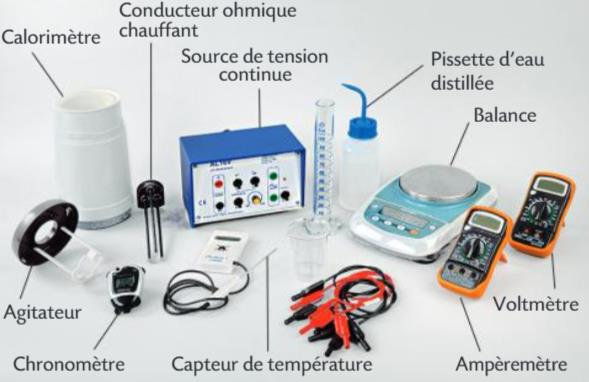
\includegraphics[width=\linewidth]{Ressources/TSPE_C14_AE_Fig1.png}
	\end{center}
\end{minipage}
\begin{minipage}{\linewidth}
	\textbf{Document 4 : Capacités thermiques}\\
	La capacité thermique d'un système combiné tel que le système \{calorimètre = eau\} est la somme des capacités thermique de chaque élément du système.\\
	\emph{Données :}
	\begin{itemize**}
		\item \textbf{Capacité thermique du calorimètre :} $C_{vase}$ = \SI{80}{\joule\per\kilo\gram}
		\item \textbf{Capacité thermique massique de l'eau : }$c_{eau}$ = \SI{4,18}{\kilo\joule\per\kelvin\per\kilo\gram}
	\end{itemize**}
\end{minipage}
\end{minipage}

\noindent \begin{minipage}{.98\linewidth}
	\textbf{Document 5 : Énergie interne et température}\\
	La variation d'énergie interne d'un système incompressible est proportionnelle à sa variation de température. Le coefficient de proportionnalité correspond à la capacité thermique $C$ du système. On a la relation :
	\begin{center}
		$\Delta U = C \times \Delta T$
	\end{center} $\Delta U$ : Variation d'énergie interne (en J) ; $C$ : Capacité thermique (en \unit{\joule\per\kelvin})
		 ; $\Delta T$ : Variation de température (en K)
\end{minipage}

\subsection*{Questions :}
\begin{enumerate}
	\item Sans faire de calcul, justifier que l'énergie interne $U$ du système augmente lorsqu'il est mis en chauffe.
\end{enumerate}
\emph{Nous allons maintenant déterminer cette variation d'énergie interne. Deux méthodes différentes sont utilisées.}\\
\textbf{\underline{Méthode 1 : }}
\begin{enumerate}[resume]
	\item Représenter sur un schéma les transferts d'énergie liés au système
	\item Écrire alors le premier principe de la thermodynamique pour ce système.
	\item Exprimer la variation d'énergie interne $\Delta U_1$ en fonction de grandeurs mesurables.
\end{enumerate}

\textbf{\underline{Méthode 2 : }}
\begin{enumerate}[resume]
	\item Exprimer la variation d'énergie interne $\Delta U_2$ du système en fonction de la température initiale et de la température finale du système.
\end{enumerate}
\begin{center}
	\textsc{\textbf{Appel N°1}}
\end{center}

\textbf{\underline{Expérience : }}
\begin{enumerate}[resume]
	\item Lister les différentes mesures à effectuer au cours de l'expérience pour déterminer la variation d'énergie interne du système \{calorimètre+ eau\} lors de don chauffage selon les deux manières étudiées précédemment.
	\item Compléter le protocole ci-dessous en conséquence
\end{enumerate}
\noindent \fbox{\begin{minipage}{.98\linewidth}
	\textbf{Protocole}
	\begin{itemize}
		\setlength\itemsep{1.5em}
		\item Tarer le calorimètre, puis y introduire environ \SI{350}{mL} d'eau.
		\item Plonger le conducteur ohmique chauffant dans l'eau.
		\item Brancher le conducteur ohmique en série avec le générateur de tension variable
		\item Allumer le générateur.
		\item Au cours de l'expérience :
		\begin{itemize}
			\item agiter régulièrement
			\item suivre l'évolution de la température
			\item contrôler que l'intensité du courant soit stable, si besoin, l'ajuster en modifiant la valeur de la tension 
		\end{itemize}
	\item Lorsque la température atteint \SI{5}{\celsius} de plus que la température initiale, stopper le chronomètre et arrêter l'expérience.
	\end{itemize}
\end{minipage}}

\begin{center}
	\textsc{\textbf{Appel N°2}}
\end{center}
\begin{enumerate}[resume]
	\item Réaliser l'expérience en prenant soin d'effectuer toutes les mesures nécessaires.
	\item Calculer les valeurs expérimentales $\Delta U_1$ et $\Delta U_2$.
	\item Comparer les deux valeurs obtenues et commenter.
\end{enumerate}

\begin{center}
	\textsc{\textbf{Appel N°3} \\
	Éteindre et ranger le matériel}
	
\end{center}

\end{document}